\documentclass[11pt,a4paper]{article}

\usepackage[T1]{fontenc}
\usepackage[utf8]{inputenc}
\usepackage[english]{babel}
\usepackage{lmodern}
%\usepackage{circuitikz}
\usepackage{color}
\usepackage{wrapfig}
\usepackage{placeins}
\usepackage{subfigure}
\usepackage{tabu}
\usepackage{fullpage}
\usepackage[squaren]{SIunits}
\usepackage{graphicx}
%\usepackage[pdftex]{graphicx}
\usepackage{epstopdf}
\usepackage{epsfig}
\usepackage{hyperref}
\usepackage{tikz}
\usepackage{tikz-qtree}
\usepackage{eurosym}
%\usepackage{chemist}
\usepackage{amsmath}
\usepackage{amssymb}
\usepackage{mathrsfs}
\usepackage{dsfont}% use $\mathds{1}$
\newcommand{\C}{\mathbb{C}}
\newcommand{\N}{\mathbb{N}}
\newcommand{\Z}{\mathbb{Z}}
\newcommand{\R}{\mathbb{R}}
\newcommand{\red}{\textcolor{red}}
\newcommand{\dis}{\displaystyle}
\newcommand{\dr}{\partial}
\newcommand{\txt}{\text}
\newcommand{\td}{\todo[inline]}
\newcommand{\ttt}{\texttt}
\newcommand{\itt}{\textit}

\usepackage{algorithm}
\usepackage{todonotes}
\usepackage[noend]{algpseudocode}

%\newtheorem{theoreme}			     {Théorème}	[chapter]
%\newtheorem{proposition}[theoreme]	 {Proposition}	
%\newtheorem{corollaire}	  [theoreme]	 {Corollaire}	
%\newtheorem{lemme}	      [theoreme]  {Lemme}		
%\newtheorem{definition}	         {Définition}[chapter]
%\theoremstyle{definition}
%\newtheorem{exemple}			     {Exemple}	[chapter]
%\newtheorem{contreexemple}[exemple]{Contre-exemple}
%\newtheorem{probleme}	             {Probl\`eme}[chapter]

\usepackage{listings}
\usepackage{textcomp}
\definecolor{listinggray}{gray}{0.9}
\definecolor{lbcolor}{rgb}{0.9,0.9,0.9}
\lstset{
	backgroundcolor=\color{lbcolor},
	tabsize=4,
	rulecolor=,
	language=matlab,
        basicstyle=\scriptsize,
        upquote=true,
        aboveskip={1.5\baselineskip},
        columns=fixed,
        showstringspaces=false,
        extendedchars=true,
        breaklines=true,
        prebreak = \raisebox{0ex}[0ex][0ex]{\ensuremath{\hookleftarrow}},
        frame=single,
        showtabs=false,
        showspaces=false,
        showstringspaces=false,
        identifierstyle=\ttfamily,
        keywordstyle=\color[rgb]{0,0,1},
        commentstyle=\color[rgb]{0.133,0.545,0.133},
        stringstyle=\color[rgb]{0.627,0.126,0.941},
}

\DeclareMathOperator{\e}{e}

\title{Titre}
\author{David Weicker}
\date{\today}

\begin{document}
\tabulinesep=1.2mm
\begin{center}
\hrule
\begin{tabular}{c}
\\[0.005cm]
\Large{Applied Numerical Methods : LAB8}\\[0.3cm] %THIS IS THE TITLE
\textsc{Goyens} Florentin  \& \textsc{Weicker} David\\[0.2cm]
$\text{10}^{\text{th}}$ December 2015\\[0.2cm] %THIS IS THE DATE
\end{tabular}
\hrule
\end{center}

\section*{Introduction}
 This report presents results for the eighth lab for the course Applied Numerical Method. The problem consists of computing the solution of an underdetermined system using SVD decomposition. 
 
 The system to solve comes from the numerical discretization of the Fredholm's integral equation and will sometimes be truncated to a certain rank $r$.
 
 \section*{Building the system}
The first thing to do is to build the linear system to be solved. The system will come from the discretization of an integral. 

Let us define the unknowns. Because we are working on the interval $[0,6]$ with $N=60$ intervals, with a constant stepsize $h=\frac{6}{N}=0.1$, we have that the unknows are an approximation of the function $p$ at different point, i.e. : 
$$p_i \approx p(x=ih)$$

That gives 61 unknows ($p_0,p_1,...,p_N,p_{N+1}$). But as stated in the homework, the function $p(x)$ is zero outside $a<x<b$ so we can conclude that $p(a)=p(0)=0$ and $p(b)=p(6)=0$. And therefore, $p_0=p_{N+1}=0$. That leaves 59 unknowns as predicted ($p_1,p_2,...,p_N$).

We secondly have to build the matrix A. It comes from the discretization of the integral using the trapezoidal rule. We have data from 36 measurements, so 36 equations and each is given by (where $K$ is the kernel function given) : 
\begin{align*}
\int_0^{6}K(x,y_i)p(x)dx &=\sum_{j=0}^{59} \int^{h(j+1)}_{hj} K(x,y_i)p(x)dx\\
&\approx \sum_{j=0}^{59} \frac{1}{2h}(K(hj,y_i)p_j+K(h(j+1),y_i)p_{j+1})\\
&=\frac{1}{h}\sum_{j=1}^{59} K(hj,y_i)p_j
\end{align*}

The last equality is found because $p_0=p_{N+1}=0$. So the matrix $A$ can be defined by : 
$$A=[a_{ij}]$$
$$a_{ij} = \frac{1}{h}K(hj,y_i)$$
$$\text{for }i=1,...,36 \text{ and }j=1,...59$$

The next thing to do is get the data vector $f=(f(y_1),...,f(y_{36}))^T$. In "real" applications, $f$ is the measured data. But here, we will generate it from the given function $p$ (and sometimes add some perturbations). In order to do this, we suppose that the $f(y)$ is a good modeling of our measuring device.

\begin{align*}
f_i&=f(y_i)=\int_0^{6}K(x,y_i)p(x)dx\\
&=\int_0^{6}K(x,y_i)(0.8cos(\pi\frac{x}{6})-0.4cos(\pi\frac{x}{2})+1)dx
\end{align*}

This integral could be performed analytically but we used the Matlab built-in function $integral$ instead (which is practically the same since the absolute tolerance of this function is $10^{-10}$). The subfunction $data$ (available at the end of this report) performs this integration and returns a vector containing the simulated data $f$.

This yields the following system to be solved in the next section : 
$$Ap=f$$ 
 
 \section*{SVD factorization for solving the system}
sqsqs
\subsection*{Adding perturbations}

We are now going to introduce some noise on the measured data. So our vector $f$ is redefined for $i=1,...,36$ by :
\begin{align*}
f_i&=f(y_i)+g_i 
\end{align*}

Where $g_i$'s come from a normal distribution with standard deviation 0.01. 

The Matlab code $svdPert.m$ (available at the end of the report) contains the code used to obtain the plots presented here.

\begin{figure}
\begin{center}
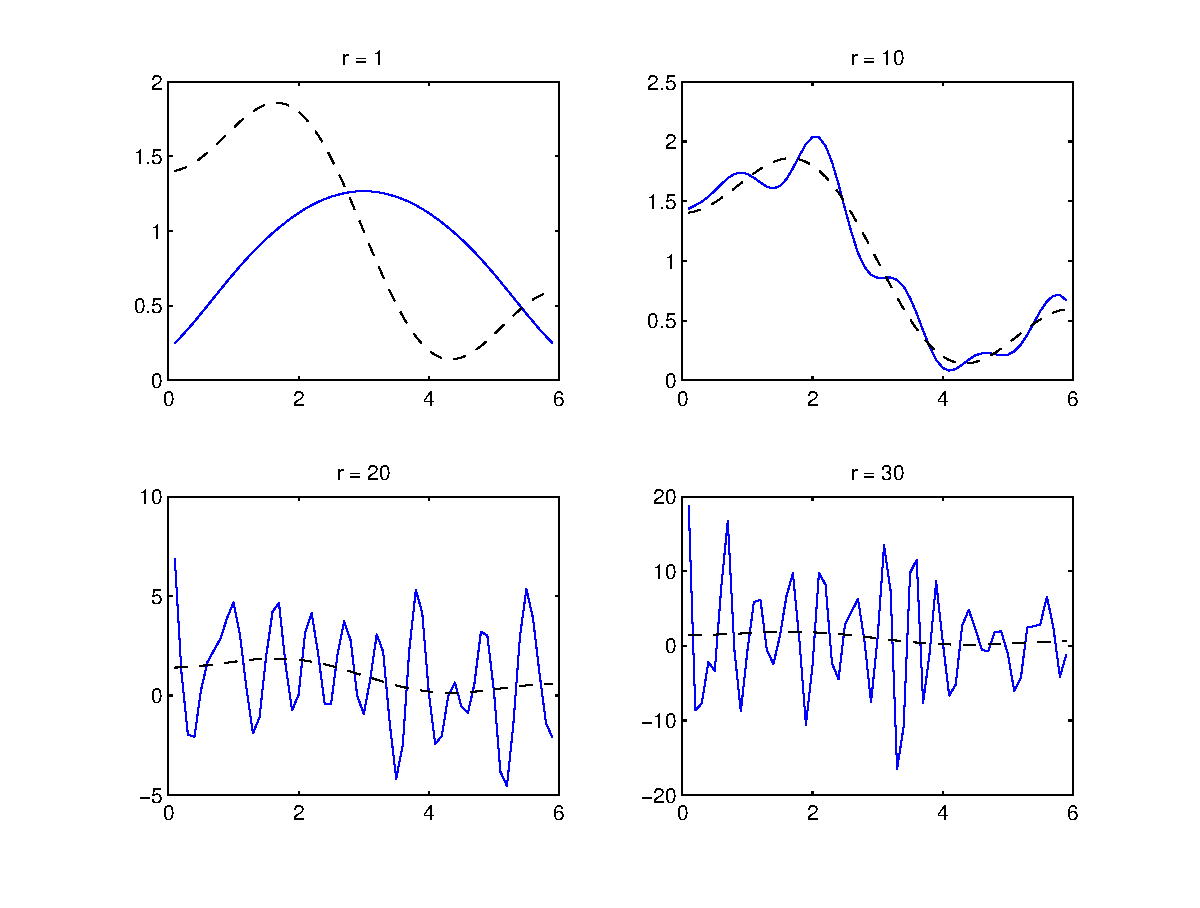
\includegraphics[scale=0.5]{perturb.eps}
\caption{Results for some values of $r$ with perturbations}
\label{perturb}
\end{center}
\end{figure}

Figure \ref{perturb} shows the solution computed with the same values of $r$ as for the problem without any perturbation. Comparing to figure \ref{fig:nn0}, we can see that for the lower values of $r$ ($r=1$ or $r=10$), the approximation is quite similar. 

On the other hand, for $r=20$ and $r=30$, adding perturbations greatly affect the quality of the solution. This is because the problem is ill-posed and thus small variations on the vector $f$ will greatly influence the solution.

Because of the perturbations, we feel, after looking at graphs for different ranks $r$, that the "best" approximation is when $r=7$. Figure \ref{rank7} shows the plot.

\begin{figure}
\begin{center}
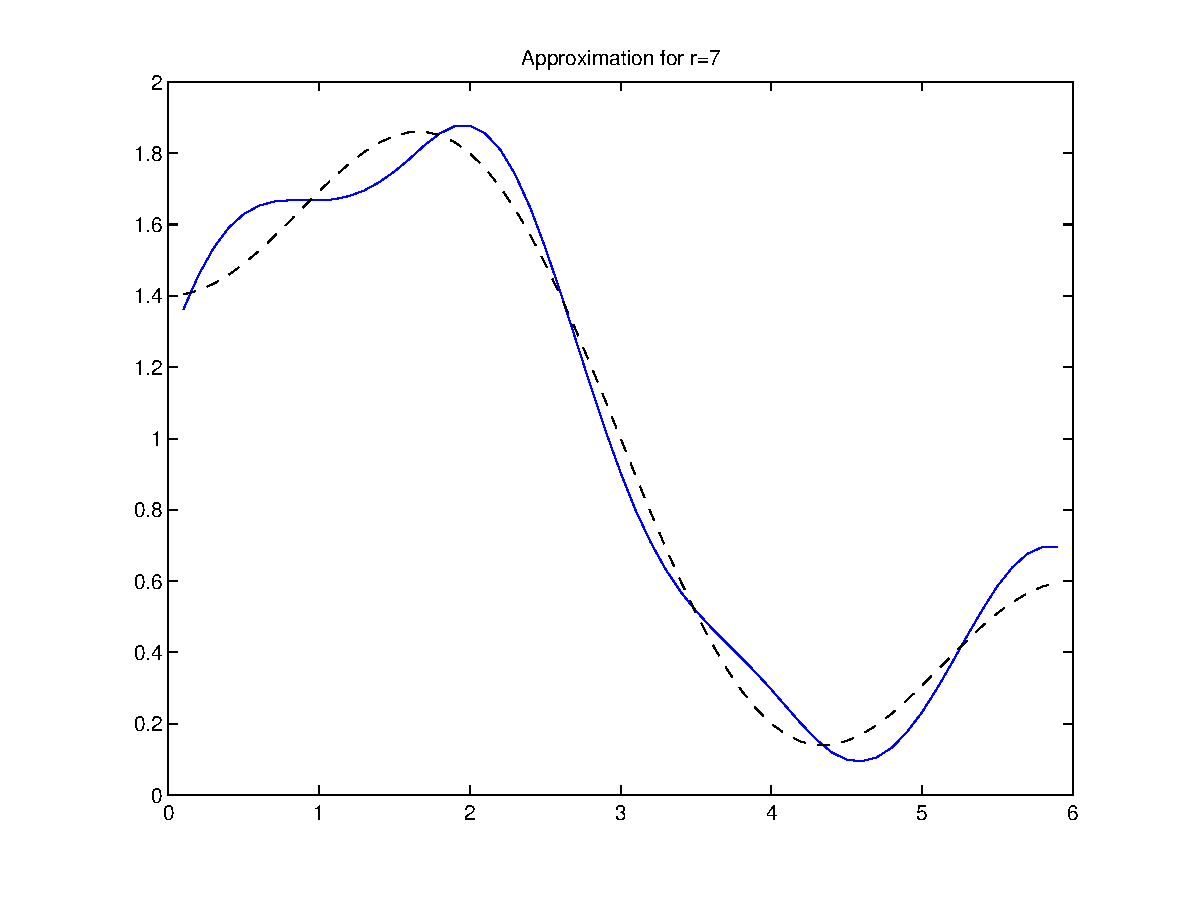
\includegraphics[scale=0.5]{rank7.eps}
\caption{Approximation for $r=7$ with noise}
\label{rank7}
\end{center}
\end{figure} 

We can note here that, because $r=7$, we are only using 7 singular values (out of the 36 possible!). Although this might seem low, we can see that the approximation is quite good. We note that adding noise forces us to reduce the rank to avoid oscillations.
\end{document}